\chapter{Methods}
\label{chapter:methods}
In the following, we present a model for the transmission of methylation patterns by \acp{DNMT}, depending on four parameter, which characterize the function of these \acp{DNMT}. Based on that, two computational methods are provided to identify the most realistic way to choose the parameters compared to some real-world methylation data. The aim of this paper is not only to compute the model parameters, but also to compare different approaches to retrieve and evaluate them.

\section{Model}
\label{Model}
The model underlies the following procedure:
\begin{enumerate}
\item initially a double-stranded, partially methylated DNA sequence with multiple \acp{CpG} is given
\item one of the strands serves as template for the methylation of a second yet unmethylated strand
\item the three \acp{DNMT} DNMT1, DNMT3a and DNMT3b eventually bind and methylate along the DNA strand
\item the cell divides and step three starts again
\end{enumerate}
Basically, each \ac{bp} is one state of the model, in which the binding state of the \acp{DNMT}is kept and if this position is part of a \ac{CpG}. If the second condition holds, the current methylation state is stored. It is assumed, there are four possible methylation states for one \ac{CpG}/\ac{CpG}-dyad. Either none of the cytosines are methylated, then the dyad is unmethylated or the cytosine at the parental or daughter strand is methylated and the respectively other one not, then the \ac{CpG} is called hemimethylated. In the final case, both cytosines are methylated, which corresponds to a fully methylated dyad. The methylation states are encoded in the following way:\newline
\begin{align}
m_i := \text{methylation state of dyad i}\\
m_i = \left\{
\begin{array}{l}
\text{0 unmethylated} \\
\text{1 hemimethylated, methylation on parent strand} \\
\text{2 hemimethylated, methylation on daughter strand} \\
\text{3 fully methylated}
\end{array}
\right.
\end{align}

\begin{figure}[h]
\centering
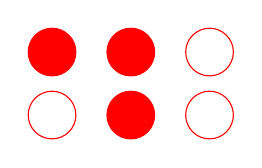
\begin{tikzpicture}
  \draw[red, fill=red](-1,0)circle(2ex);
  \draw[red](-1,-0.8)circle(2ex);
  \draw[red, fill=red](0,0)circle(2ex);
  \draw[red, fill=red](0,-0.8)circle(2ex);
  \draw[red](1,0)circle(2ex);
  \draw[red](1,-0.8)circle(2ex);
\end{tikzpicture}
\caption{A methylation pattern with three CpGs; each circle represents one CpG; plane red circles are methylated CpGs; the pattern code is 28 and is computed as $1*4^2 + 3*4^1 + 0*4^0 = 16 + 12 + 0 = 28$}
\label{fig:mexample}
\end{figure}

The different methylation patterns in figure \ref{fig:methylationpatterns}, whereby subfigure \ref{fig:sfig0} corresponds to pattern 0 and so on.\newline
In this way, the full methylation pattern of a DNA sequence can be encoded as a number in range $4^(L-1)$, where L is the number of \acp{CpG}. The code can be interpreted as sum over the methylation states. Hereby the rightmost dyad is the zeroth dyad and all following methylation states are shifted by 2 bits times the enumeration of the dyad (see an example in figure \ref{fig:mexample}).
\[\sum^{L-1}_{i=0}{m_i * 4^{L-1-i}}\]
\begin{figure}
\{0:0.2, 1:0.01, 3:0.02, 11:0.1, 14:0.05, 35:0.01, 36:0.21, 56:0.15, 57:0.05, 63:0.2\}
\label{dict}
\caption{methylation pattern distribution of a locus with 3 CpGs; each key represents one methylation pattern, the following number the frequency of this pattern; the patterns not listed have frequency zero; assuming, there are 100 samples, the patterns have a absolute frequency of 20, 1, 2, 1, 5, 1, 21, 15, 5 and 2 respectively.}
\end{figure}
If we are given a set of methylation patterns, the pattern distribution may be represented as dictionary, where the key of each entry is a methylation pattern and its value the frequency of this key in the set of methylation patterns. See Figure \ref{dict} for an example.\\

Further, it is assumed two methyltransferases are active, DNMT1 and DNMT3. For simplification, no other enzymes are included in the model, thus there may be enzymes which influence the methylation process. In earlier experiments it was shown that DNMT1 binds to the daughter strand, whereas DNMT3 is able to bind to both strands (see section \ref{section:DNAMeth}). This knowledge is included by recognizing the binding state of each enzyme to their strands.\newline
Therefore, each state of a \ac{CpG} can be stored as a combination of four numbers, where the numbers contribute to the methylation state, the binding state of DNMT1 to the new strand and DNMT3 to the old and new strand respectively.
\begin{align*}
S_i := \text{state of dyad i}\\
S_i = (m_i, B1_i, B3p_i, B3d_i)\\
m \in \{0,1,2,3\}^L\\
B1 \in \{0,1\}^L\\
B3p \in \{0,1\}^L\\
B3d \in \{0,1\}^L
\end{align*}
Here B1 is the binding state of DNMT1 and B3p the binding state of DNMT3 to the parental strand and B3d the binding state to of DNMT3 to the daughter strand. Zero and one signify an unbound and bound enzyme.\\

%de novo/maintenance
\begin{figure}[h]
\centering
\begin{tikzpicture}[>=stealth',bend angle=45,auto,->,shorten >=1pt]
  \tikzstyle{place}=[circle,thick,draw=black!75,minimum size=6mm,font=\large]
  \node [place](0)at (0,0){0};
  \node [place](1)at (1.5,0.8){1};
  \node [place](2)at (1.5,-0.8){2};
  \node [place](3)at (3,0){3};
  \path (0)edge node{$\delta$}(1)
  		   edge node{$\delta$}(2)
  		(1)edge node{$\mu$}(3)
  	    (2)edge node{$\mu$}(3);
\end{tikzpicture}
\caption{Possible transitions between the methylation patterns of a dyad; the numbers represent the methylation patterns m; each transition shows a possible methylation with the probability denoted on the arrow}
\label{mhy}
\end{figure}
Two kinds of methylations are distinguished in the model. The methylation of a cytosine is called maintenance if the opposite base is yet methylated. Contrary, if the opposite base is unmethylated, the methylation event is called de novo. And the probabilities of each event are denoted by $\mu$ and $\delta$, consistent to earlier approaches (\ref{section:RelWork}). Figure \ref{mhy} shows the resulting possible transitions.\\

%rho/tau
\begin{figure}[h]
\centering
\begin{tikzpicture}[>=stealth',bend angle=45,auto,shorten >=1pt]
  \tikzstyle{place}=[circle,thick,draw=black!75,minimum size=6mm,align=center]
  \tikzstyle{red}=[circle,thick,draw=red!75,minimum size=6mm,align=center, text=red]
  \draw[thick] (0,0) -- (9,0) node[anchor=north west]{position(bp)};
  \foreach \x in {0,1,2}
   \draw (\x *3+1,1pt) -- (\x *3+1,-1pt) node[anchor=north] {$\x$};
  \node [place](0u)at (1,4){DNMT\\ unbound};
  \node [place](1u)at (4,4){DNMT\\ unbound};
  \node [place](2u)at (7,4){DNMT\\ unbound};
  \node [red](0b)at (1,1){DNMT\\ bound};
  \node [red](1b)at (4,1){DNMT\\ bound};
  \node [red](2b)at (7,1){DNMT\\ bound};
  \path[->] (0b)edge node{$\rho$}(0u)
  		   edge node{$1-\rho$}(1b)
  		(1b)edge node{$\rho$}(1u)
  		   edge node{$1-\rho$}(2b)
  		(2b)edge node{$\rho$}(2u)
  		(0u)edge node{$1-\tau$}(1u)
  			edge node{$\tau$}(1b)
  		(1u)edge node{$1-\tau$}(2u)
  			edge node{$\tau$}(2b);
\end{tikzpicture}
\caption{Transitions between the binding states of a DNMT over the DNA; each number represents one bp on the strand; red circles symbolize that DNMT is bound to the DNA at that position, black ones are unbound enzymes; the arrows show possible transitions between the binding states}
\label{rho}
\end{figure}
The probabilities of attachment and disattachment of a \ac{DNMT} are defined as $\tau$ and $\rho$. Therefore, the association length, the number of \acp{bp} where the enzyme is bound is $1/\rho$ and the probability that the \ac{DNMT} stays bound at one \ac{bp} and its neighbour is 1-$\rho$. This parameter setting is similar to the approach of Fu et al. from 2012.\cite{Fu} Figure \ref{rho} visualises the binding states and their probabilities.\\

%Alle Übergänge 
\begin{figure}[h]
\begin{tabularx}{\textwidth}{l|c|c|c|c}
\multicolumn{5}{c}{\textbf{$m_i$}}\\
\cline{2-5}
\textbf{($m_i, B1_i, B3p_i, B3d_i$)}&	0&	1&	2&	3\\
\hline
(0, 0, 0, 0)&	1&	0&	0&	0\\
(0, 0, 0, 1)&	$1-\delta_d$&	0&	$\delta_d$&	0\\
(0, 0, 1, 0)&	$1-\delta_p$&	$\delta_p$&	0&	0\\
(0, 0, 1, 1)&	$(1-\delta_p)(1-\delta_d)$&	$\delta_p(1-\delta_d)$&	$\delta_d(1-\delta_p)$&	$\delta_p \delta_d$\\
(0, 1, 0, 0)&	1&	0&	0&	0\\
(0, 1, 0, 1)&	$1-\delta_d$&	0&	$\delta_d$&	0\\
(0, 1, 1, 0)&	$(1-\delta_p)$&	$\delta_p$&	0& 0\\
(0, 1, 1, 1)&	$(1-\delta_p)(1-\delta_d)$&	$\delta_p(1-\delta_d)$&	$\delta_p(1-\delta_d)$&	$\delta_p \delta_d$\\
(1, 0, 0, 0)&	0&	1&	0&	0\\
(1, 0, 0, 1)&	0&	$1-\delta_d$&	0&	$\delta_d$\\
(1, 0, 1, 0)&	0&	1&	0&	0\\
(1, 0, 1, 1)&	0&	$1-\delta_d$&	0&	$\delta_d$\\
(1, 1, 0, 0)&	0&	$1-\mu$&	0&	$\mu$\\
(1, 1, 0, 1)&	0&	$(1-\mu)(1-\delta_d)$&	0&	$\mu+\delta_d$\\
(1, 1, 1, 0)&	0&	$1-\mu$&	0& $\mu$\\
(1, 1, 1, 1)&	0&	$(1-\mu)(1-\delta_d)$&	0&	$\mu+\delta_d$\\
\end{tabularx}
\caption{Transition probabilities between the methylation states; $m_i$ on the left side is the methylation state before DNMT activity, either unmethylated(0) or methylated on the parent strand(1), the four rightmost columns represent the four possible methylation states after DNMT activity; the other three parameters in the leftmost column are the binding state of the three different DNMTs; B1 - DNMT1, B3p - DNMT3 at parental strand, B3d - DNMT3 on daughter strand, where 0 means disassociated and 1 associated; later disassociation and association rates are not included in the probabilities; $\mu$ is the maintenance methylation probability of DNMT1, $\delta_p$ the de novo methylation probability of DNMT3 on the parental strand and $\delta_d$ on the daughter strand.}
\label{allProbs}
\end{figure}
Further assumptions for our model are that DNMT1 methylates before DNMT3 as results of \cite{Lueck} suggested this ordering as the most probable and that DNMT1 performs mainly maintenance methylation, whereas DNMT3 is specialized on de novo methylation. Figure \ref{allProbs} shows the different combinations of transitions that may lead from one methylation state to another, given the methylation state of the dyad before any methylation activity and the binding states of the three \acp{DNMT}. The start methylation state can either be unmethylated or methylated on the parental strand because the newly synthesized strand is initially unmethylated. In this table it is assumed that disassociation and association events have taken place and are excluded in the transition matrix. Because our model does not include demethylation events, a transition from methylated to unmehtylated is not possible.\\

\section{Simulation}
\label{sim}
\textbf{\textsc{Problem:}} \ac{DNMT} simulation\newline
\textbf{Given:} initial methylation pattern distribution $X_0$, parameters $\rho, \tau, \mu$ and $\delta$\newline
\textbf{Goal:} generate methylation pattern distribution at time $t$, $X_t$\\

\begin{figure}[h]
\begin{tabularx}{\textwidth}{l|c|c}
$m_i$&	$u_i$&	$l_i$\\
\hline
0&	0&	0\\
1&	1&	0\\
2&	0&	2\\
3&	1&	2\\
\end{tabularx}
\label{celldiv}
\caption{methylation states before and after cell division; $m_i$ - before cell division, $u_i$ - the upper strand serves as new parental strand, $l_i$ - lower strand is new parental strand.}
\end{figure}
To initialize our model, the methylation pattern of one DNA-strand at time zero before any replication is needed. We receive one random methylation pattern by drawing from the initial pattern distribution (see \ref{Model}). The number drawn represents the methylation pattern of a double stranded DNA with multiple \acp{CpG}. Now, the first cycle of replication starts by cell division; the strands separate and a new, unmethylated strand is synthesized. In figure \ref{celldiv} the transitions between the previous double-stranded DNA and the two resulting double-strands are shown. In our simulation we randomly choose between the two methylation patterns with probability 0.5.

\section{MLE}
\label{MLE}

\section{ABC}
\label{ABC}